\section{Theorie}
\label{sec:Theorie}
\subsection{Der RCL-Schwingkreis}
\label{sec:RCL}
Ein Schwingkreis ist eine elektrische Schaltung, bei welcher Energie in Form eines elektrischen Stroms zwischen zwei Energiespeichern hin 
und her oszillieren. Diese Energiespeicher sind gegeben durch eine Induktivität $L$ und einen Kondensator $C$. Bei einem CL-Kreis gilt dabei
Energieerhaltung, die Schwingung wird also nicht gedämpft. Wird in die Schaltung jedoch ein ohmscher Widerstand $R$ eingebaut, so geht über 
diesen Energie in Form von Wärme verloren, die Energie ist im Schwinkreis also nicht mehr erhalten. Ein solcher RCL-Schwinkreis führt demnach
gedämpfte Schwingungen aus.\\\noindent
Zusätzlich kann noch eine Spannungsquelle hinzugefügt werden, sodass dem Schwingkreis Energie zugeführt wird. Ein solcher getriebener 
Schwingkreis führt dann gezwungene Schwingungen aus. Der Aufbau der beiden Schwingkreise ist in den Abbildungen \ref{fig:gedampft} und 
\ref{fig:getrieben} noch einmal skizziert.
\begin{figure}[H]
    \begin{minipage}[b]{.5\linewidth} % [b] => Ausrichtung an \caption
       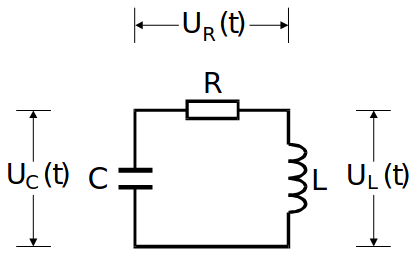
\includegraphics[width=\linewidth]{pictures/gedampft.png}
       \caption{Der gedämpfte Schwingkreis. \cite{AP01}}
       \label{fig:gedampft}
    \end{minipage}
    \hspace{.1\linewidth}% Abstand zwischen Bilder
    \begin{minipage}[b]{.4\linewidth} % [b] => Ausrichtung an \caption
       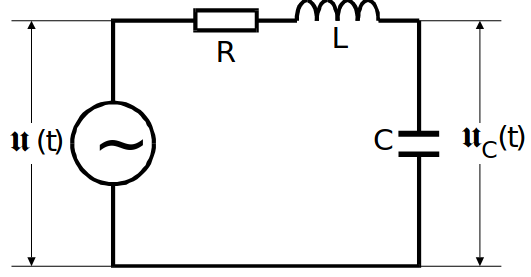
\includegraphics[width=\linewidth]{pictures/getrieben.png}
       \caption{Der getriebene Schwingkreis. \cite{AP01}}
       \label{fig:getrieben}
    \end{minipage}
  \end{figure}
\noindent
Im Folgenden werden diese beiden Schwinkreise näher beleuchtet.

\subsection{Gedämpft Schwingungen}
\label{sec:gedämpft}
Um die Differentialgleichung für einen gedämpften Schwinkreis zu erhalten, wird von dem 2. Kirchhoffschen Gesetz
\begin{equation}
    U_R(t)+U_C(t)+U_L(t)=0
    \label{eqn:kirchhoff2}
\end{equation}
mit
\begin{align*}
U_R(t)&=RI(t)                           \\
U_C(t)&=\frac{Q(t)}{C}                  \\
%U_L(t)&=L\frac{\text{d}I(t)}{\text{d}t}
U_L(t)&=L\dot{I}    
\end{align*}
ausgegangen. Mit dem Zusammenhang 
\begin{equation*}
    I=\frac{dQ}{dt}
\end{equation*}
kann durch Einsetzen in das 2. Kirchhoffsche Gesetz \eqref{eqn:kirchhoff2} und durch einmaliges Ableiten nach der Zeit
die Differentialgleichung
\begin{equation}
    \ddot{I}+\frac{R}{L}\dot{I}+\frac{1}{LC}I=0
    \label{eqn:DGL1}
\end{equation}
erhalten werden. Die Lösung der Differentialgleichung ist dabei gegeben durch
\begin{equation}
    I=e^{-2\pi\mu t}\left(Ae^{i2\pi\nu t}+Be^{-i2\pi\nu t}\right), \qquad A,B\in\mathbb{C}
    \label{eqn:Losung1}
\end{equation}
mit
\begin{equation*}
    2\pi \mu=\frac{R}{2L} 
    \qquad\text{und}\qquad 
    2\pi \nu=\sqrt{\frac{1}{LC}-\frac{R^2}{4L^2}} .
\end{equation*}
Auflösen der ersten Gleichung nach $R$ liefert den effektiven Dämpfungswiderstand 
\begin{equation}
    R_{eff}=4\pi\mu L 
    \label{eqn:Reff}
\end{equation}
Offensichtlich wird $\nu$ für $1/LC<R^2/(4L^2)$ komplex, weswegen in einer Fallunterscheidung drei Möglichen Fälle 
diskutiert werden.

\subsubsection*{1.Fall: $1/LC>R^2/(4L^2)$}
In dem ersten Fall ist $\nu$ reell und somit die Exponentialfunktionen in \eqref{eqn:Losung1} komplex. Damit die Lösung trotzdem reell ist muss
für die Konstanten $A=B^{*}$ gelten. Somit wird \eqref{eqn:Losung1} zu
\begin{equation*}
    I=A_0E^{-2\pi\mu t} cos(2\pi\nu t+\eta).
    \label{eqn:Fall1}
\end{equation*}
Wie in Abbildung \ref{fig:Fall1} zu erkennen ist, handelt es sich bei dieser Lösung um eine gedämpfte Schwingung, die mit zunehmender Zeit 
exponentiell gegen 0 geht. Die Schwingungsdauer ist dabei gegeben durch
\begin{equation*}
    T=\frac{1}{\nu} ,
\end{equation*}
$\nu$ ist also eine Frequenz. Die Abklingdauer ist dabei beinahe analog
\begin{equation}
    T_{ex}=\frac{1}{2\pi\mu}
    \label{eqn:Tex}
\end{equation}
\begin{figure}[H]
    \centering
    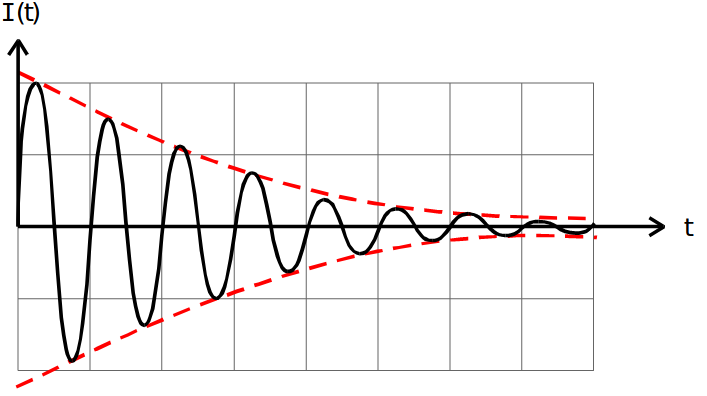
\includegraphics[width=0.7\textwidth]{pictures/Fall1.png}
    \caption{Die Stromstärke als Funktion der Zeit für $1/LC>R^2/(4L^2)$. Die einhülende Exponentialfunktion ist in rot skizziert.\cite{AP01}}
    \label{fig:Fall1}
\end{figure}

\subsubsection*{2.Fall: $1/LC<R^2/(4L^2)$}
In diesem Fall ist $\nu$ rein imaginär, die Exponentialfunktionen in \eqref{eqn:Losung1} sind also alle reell. Demnach findet keine Oszillation
statt, wie in Abbildung \ref{fig:Fall2} zu sehen ist. Dabei kann die Funktion sowohl das Vorzeichen welchseln (vgl. grün \ref{fig:Fall2}), als
auch Extremwerte annehmen (vgl. rot, grün \ref{fig:Fall2}) oder monoton gegen null fallen (vgl. blau \ref{fig:Fall2}). Der Grenzwert für lange
Zeiten liegt jedoch immer bei null. Es gilt dabei
\begin{equation*}
    I(t)\propto \exp\left(\left(\frac{R}{2L}-\sqrt{\frac{R^2}{4L^2}-\frac{1}{LC}}\right)t\right)    .
\end{equation*}
\begin{figure}[H]
    \centering
    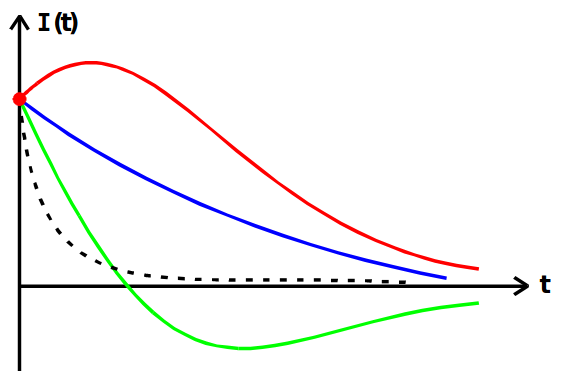
\includegraphics[width=0.6\textwidth]{pictures/Fall2.png}
    \caption{Verschiedene Verläufe der Stromstärke für $1/LC<R^2/(4L^2)$. Der aperiodische Grenzfall ist gestrichelt skizziert.\cite{AP01}}
    \label{fig:Fall2}
\end{figure}

\subsubsection*{3.Fall: $1/LC=R^2/(4L^2)$}
\label{sec:Fall3}
Dieser Fall wird auch aperiodischer Grenzfall genannt, da $\nu$ für $1/LC=R^2/(4L^2)$ gerade null ist. Dadurch vereinfacht sich \eqref{eqn:Losung1}
zu 
\begin{equation*}
    I(t)=Ae^{-\frac{t}{\sqrt{L}}}   .
\end{equation*}
Für genau diesen Fall geht die Amplitude von $I(t)$ am schnellsten gegen null, ohne dabei überzuschwingen. Der aperiodische Grenzfall ist in 
Abbildung \ref{fig:Fall2} als gestrichelte Linie eingezeichnet. 

\subsection{Erzwungene Schwingungen}
Wird der Schwingkreis an eine externe Spannungsquelle angeschlossen, können damit Schwingungen erzwungen werden. Der Aufbau eines solchen Schwinkreises
ist in Abbildung \ref{fig:getrieben} dargestellt. Die neue Differentialgleichung wird recht analog zu \eqref{eqn:DGL1} hergeleitet, wobei auf der 
rechten Seite die Spannung $U(t)=U_0\exp(i\omega t)$ der Spanungsquelle ergänzt wird. Wegen dieser wird nun auch die Spannung $U_C(t)$ auf dem Kondensator
und nicht mehr $I(t)$ betrachtet. Es ergibt sich demnach
\begin{equation*}
    LC\ddot{U}_C+RC\dot{U}_C+U_C=U_0e^{i\omega t}   .
    \label{eqn:DGL2}
\end{equation*}
Die allgemeine Lösung dieser Differentialgleichung lautet
\begin{equation}
    U(t)=\frac{U_0(1-LC\omega^2-i\omega RC)}{(1-LC\omega^2)^2+\omega^2R^2C^2}   ,
    \label{eqn:Losung2}
\end{equation}
wobei $U_C$ als reelle Messgröße mit der komplexen Gleichung \eqref{eqn:Losung2} in dem Zusammenhang
\begin{equation}
    U_C(\omega,t)=U(\omega)e^{i\omega t} 
    \label{eqn:UuUC}
\end{equation} 
stehen. Nun werden von dem komplexen $U(t)$ der Betrag $|U|$ sowie die Phase $\phi(\omega)$ gebildet:
\begin{align} %Das geht bestimmt auch schöner :(
    |U|          &= \sqrt{\Re^2(U)+\Im^2(U)}      & &=& &\frac{U_0}{\sqrt{(1-LC\omega^2)^2+\omega^2R^2C^2}} \label{eqn:ubetrag} \\
    \phi(\omega) &= \arctan{\frac{\Im(U)}{\Re(U)}}& &=& &\arctan{\frac{-\omega RC}{1-LC\omega^2}} \label{eqn:uphase}
\end{align}
Aus dem Zusammenhang \eqref{eqn:UuUC} folgt dabei, dass $U_C(\omega)=|U|$ ist. Somit beschreibt Gleichung \eqref{eqn:ubetrag} die Kondensatorspannung
$U_C$ in Abhängigkeit der Frequenz $\omega$. Es existiert nun ein $\omega$, für welches $U_C$ maximal und dabei größer als $U_0$ ist. Diese 
sogennante Resonanzfrequenz ist dabei 
\begin{equation*}
    \omega_{res}=\sqrt{\frac{1}{LC}-\frac{R^2}{2L^2}}   .
\end{equation*}
Für eine schwache Dämpfung $(R^2)/(2L^2)<<1/(LC)$ dominiert der erste Teil unter der Wurzel, sodass $\omega_{res}\approx 1/\sqrt{LC}=\omega_0$ gilt. Für die maximale Amplitude
der Kondensatorspannung folgt damit
\begin{equation*}
    U_{C, \text{max}} = \frac{1}{\omega_0 RC} U_0  .
\end{equation*}
Um das Maß der Überhöhung der Kondensatorspannung $U_C$ im Vergleich zu der Erregeramplitude $U_0$ zu beschreiben, wird der Faktor der die beiden
Größen verbindet als Güte $q$ definiert. Es gilt also
\begin{equation}
    q=\frac{1}{\omega_0RC}
    \label{eqn:gute}
\end{equation}
Als Maß für die Schärfe der Resonanz, werden die Frequenzen $\omega_-$ und $\omega_+$ als die Frequenzen definiert, bei denen das Maximum $U_C(\omega_res)$
um den Faktor $1/\sqrt{2}$ abgesunken ist. $\omega_-$ und $\omega_+$ erfüllen somit die Gleichung
\begin{equation*}
    q\frac{U_0}{\sqrt{2}}=\frac{U_0}{c\sqrt{\omega_{\pm}^2R^2+(\omega_{\pm}^2L-1/C)^2}} .
\end{equation*}
Für $R^2/L^2<<\omega_0^2$ vereinfacht sich die Gleichung zu
\begin{align*}
                    &\omega_+-\omega_-\approx \frac{R}{L} \\
    \Leftrightarrow \qquad &q=\frac{\omega_0}{\omega_+-\omega_-}    .
\end{align*}
Für eine starke Dämpfung $(R^2)/(2L^2)>>1/(LC)$ fällt $U_C$ von $U_0$ aus monoton gegen null, sodass $U_C$ die Erregeramplitude nicht überhöhen kann. 